%%% Local Variables:
%%% mode: latex
%%% TeX-master: t
%%% End:

\chapter{在某航空控制系统中的应用}
\label{cha:case}

受某研究所委托,我所在实验室为其验证在某航空控制系
统中的中断驱动程序。其中一项重要的验证需求就是验证中断优先级设置的合理性。换句话
说,需要验证中断在既有优先级的设置下,其实时性得到保障。本章应用第~\ref{cha:intr} 
章描述的方法和模型,针对本项目做了一些修改,最后完成了该验证需求。

\section{应用系统简介}
\label{sec:system_intro}

构建形式化模型之前,我们首先需要对该系统的中断实现有一个全面详细的了解。

\subsection{中断控制器介绍}
\label{subsec:8259}

\begin{figure}[H]
	\centering
	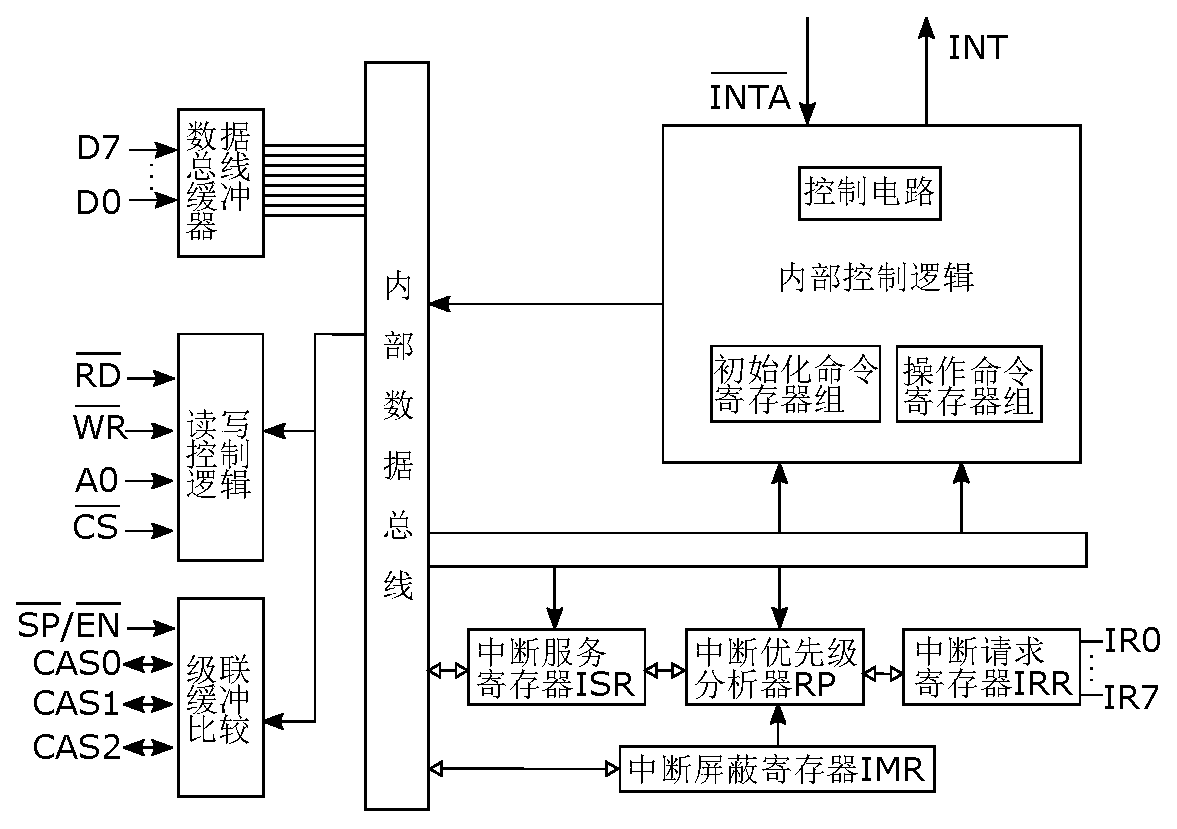
\includegraphics[width=0.9\textwidth]{8259_internal}
	\caption{8259的内部逻辑}
	\label{fig:8259_internal}
\end{figure}

该系统采用Intel 8259芯片控制中断。Intel8259是一系列可编程化中断控制器(
PIC:Programmable Interrupt Controller)芯片的总称,当初设计它是为了搭配 8-bit
的Intel 8085以及16-bit的Intel 8086等微处理器来使用。此系列的芯片原本包含 8259、
8259A、和 8259B,但时至今日,许多制造商已制作了相当多与8259兼容的芯片。运作上,
8259是一个多任务器,它会从多个中断源中挑出一个中断信号,并输出。

8259的内部结构如图~\ref{fig:8259_internal} 所示,其内部结构逻辑主要由以下三部
分组成:

\begin{itemize}
	\item 控制逻辑
	\item 中断优先权判优及其屏蔽
	\item 辅助电路
\end{itemize}

\subsubsection{编程结构}
\label{subsubsec:8259_program}

8259的编程结构共由10个寄存器构成,每个寄存器均为8位。如图~\ref{fig:8259_program}
所示。

\begin{figure}[H]
	\centering
	
\includegraphics[width=0.9\textwidth]{8259_program}
	\caption{8259的编程结构}
	\label{fig:8259_program}
\end{figure}

10个寄存器可分为三组。第一组:IRR、PR、ISR。

\begin{description}
	\item[IRR] 中断请求寄存器(Interrupt Request Register) 该寄存器的8位(D
	7~D0)分别存放IR7~IR0输入线上的中断请求。当某输入线有请求时,IRR对应位置1,
	该寄存器具有锁存功能。
	\item[ISR] 当前中断服务寄存器(In Service Register) 该寄存器用于存放正在
	被服务的所有中断级,包括尚未服务完而中途被别的中断打断了的中断级。
	\item[PR] 优先级裁决器(Priority Resolver) 当IR输入线上有请求时,IRR对应
	位置1,同时,PR将该中断的优先级与ISR中的优先级比较,若该中断的优先级高于ISR
	中的最高优先级,则PR就使INT信号变为高电平,把该中断送给CPU,同时,在ISR相应
	位置1。否则,PR不为该中断提出申请。
\end{description}

第二组:ICW1、ICW2、ICW3、ICW4。这四个寄存器用来存放初始化命令字(Initialization 
Command Word)。初始化命令字一般在系统启动时由程序设置,一旦设定,一般在系统工作
过程中就不再改变。

\begin{description}
	\item[ICW1] 指定本8259是否与其他8259级联,以及中断请求输入信号的形式(边沿
	触发/电平触发)。
	\item[ICW2] 指定中断类型码。
	\item[ICW3] 指定本8259与其他8259的连接关系。
	\item[ICW4] 指定本片8259的中断结束方式、中断嵌套方式、与数据总线的连接方式
	(缓冲/非缓冲)。
\end{description}

第三组:OCW1、OCW2、OCW3。这三个寄存器用于存放操作命令字(Operation Command 
Word)。操作命令字由应用程序使用,以便对中断处理过程作动态控制。在系统运行过程中,
操作命令字可以被多次设置。

\begin{description}
	\item[OCW1] 又称中断屏蔽寄存器(IMR:Interrupt Mask register),当其某位置
	1时,对应的IR线上的请求被屏蔽。例如,若OCW1的D3位置1,当IR3线上出现请求时,
	IRR的D3位置1,但8259不把IR3的请求提交优先级仲裁器PR裁决,从而,该请求没有机
	会被提交给CPU。
	\item[OCW2] 指定优先级循环方式及中断结束方式。
	\item[OCW3] 指定8259内部寄存器的读出方式、设定中断查询方式、设定和撤消特殊
	屏蔽方式。
\end{description}

\subsubsection{功能}
\label{subsubsec:8259_function}

8259通过以下4个功能来完成中断管理器的工作。

\begin{enumerate}[(1)]
	\item 一片Intel 8259可管理8个中断请求,并把当前优先级最高的中断请求送到CPU
	的INTR端。
	\item 当CPU响应中断时,为CPU提供中断类型码。
	\item 8个外部中断的优先级排列方式,可以通过对8259编程进行指定。也可以通过编
	程屏蔽某些中断请求,或者通过编程改变中断类型码。
	\item 允许9片8259级联,构成64级中断系统。在微机中,使用两片8259级联,构成15
	级中断,其连接情况如图~所示。
\end{enumerate}

\begin{figure}[H]
	\centering
	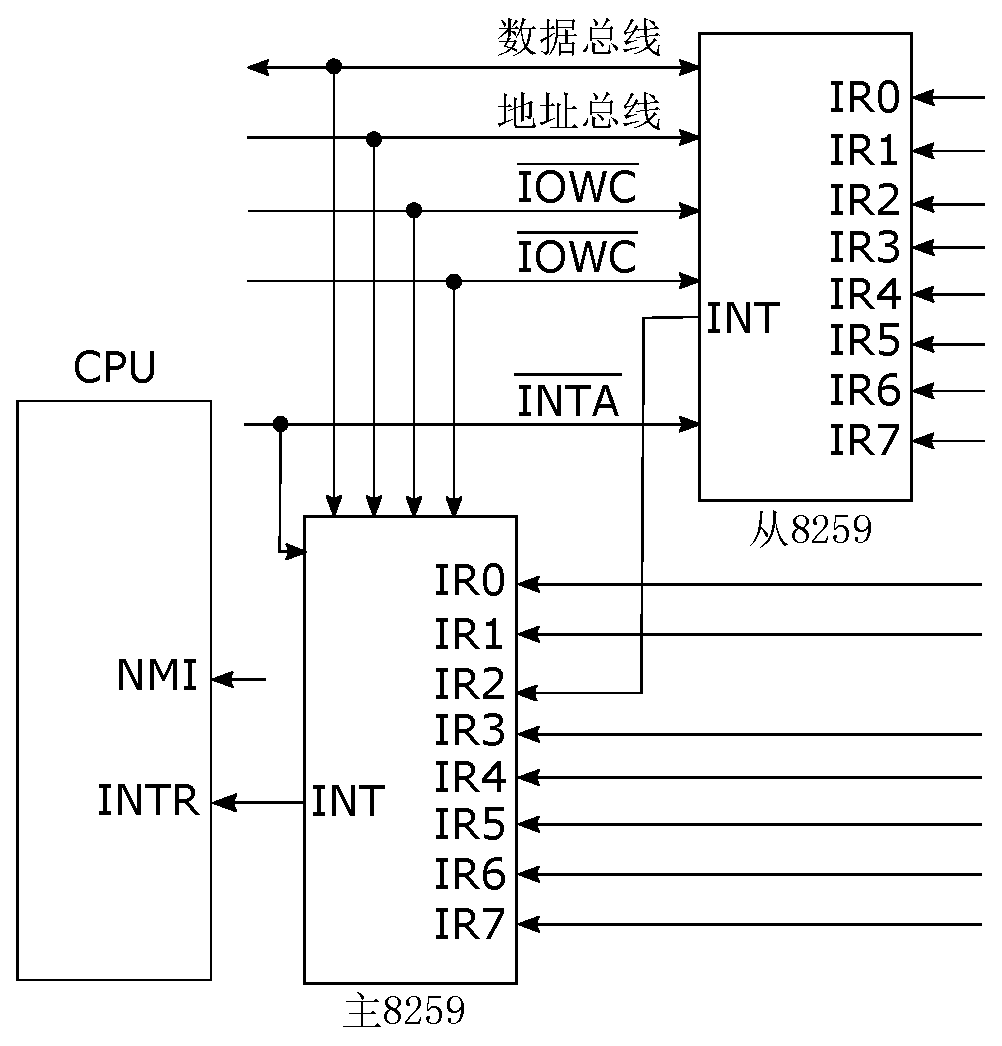
\includegraphics[width=0.6\textwidth]{8259_cascad}
	\caption{8259的编程结构}
	\label{fig:8259_cascad}
\end{figure}

\subsubsection{工作原理}
\label{subsubsec:8259_work}

8259完成一次中断处理的工作步骤如下:

\begin{enumerate}[(1)]
	\item 线上提出了中断请求的中断源,即出现请求,IRR中断请求寄存器(共有8位D7~
	D0)对应于连接在IR0~IR7线上的外设的中断请求,哪一根输入线有请求,哪一根输入
	线就置1。。
	\item 若OCW1(IMR中断屏蔽寄存器)未使该中断请求屏蔽(对应位为0时不屏蔽),
	该请求被送入PR(优先权分析器)比较。否则,不送入PR比较。	
	\item 把新进入的请求与ISR(服务中寄存器)中正在被处理的中断进行比较。如果新
	进入的请求优先级较低,则8259不向CPU提出请求。如果新进入的请求优先级较高,则
	8259使INT引脚输出高电平,向CPU提出请求。
	\item 如果CPU内部的标志寄存器中的IF(中断允许标志)为0,CPU不响应该请求。若
	IF=1,CPU在执行完当前指令后,从CPU的INTA引脚上向8259发出两个负脉冲。
	\item 第一个 INTA负脉冲到达8259时,8259完成以下三项工作:
	\begin{enumerate}[a.]
		\item 使IRR的锁存功能失效。这样一来,在IR7~IR0上的请求信号就不会被8259
		接收。直到第二个INTA负脉冲到达8259时,才又使IRR的锁存功能有效。 
		\item 使ISR中的相应位置1。
		\item 使IRR中的相应位清0。
	\end{enumerate}
	\item 第二个INTA负脉冲到达8259时,8259完成以下工作:
	\begin{enumerate}[a.]
		\item 将中断类型码(ICW2中的值)送到数据总线上,CPU将其保存在“内部暂存器”
		中。
		\item 如果ICW4中设置了中断自动结束方式,则将ISR的相应位清0。
	\end{enumerate}
	\item CPU把PSW(程序状态控制字)入栈。
	\item PSW中的IF、TF清0。
	\item CS入栈。
	\item IP入栈。
	\item 根据内部暂存器的值获得中断向量表中的位置,从中断向量表内取出一字,送
	CS。
	\item 从中断向量表内取出一字,送IP。
	\item 至此,CPU转入中断处理程序执行。在中断处理程序中,IF为0,CPU不会响应
	新的8259的请求。(同时,TF=0,不允许单步执行中断处理程序)。但在中断处理程
	序中,可以使用STI指令(开中断,使IF=1),使CPU允许响应新的8259的请求,这样
	一来,如果8259有更高优先级的请求,该中断处理程序将被中断,出现了中断嵌套。
	\item 中断处理程序的最后一条指令为IRET(中断返回)。该指令从堆栈中取出(8)
	\pozhehao (10)步保存的IP、CS、PSW,CPU接着执行被中断的程序。
\end{enumerate}

\subsection{中断设置}
\label{subsec:intr_setting}

某航空控制系统采用两片Intel 8259级联的方式,如图3所示。我们称与CPU连接的Intel 8259
为主片,与主片连接的另一片为从片。该项目中涉及中断共10个,主从片上各5个。主片上中断
优先级比从片高。主从片上中断优先级固定,没有动态变化。

10个中断中,有3个中断在实际运行中不会被触发。因此我们需要考虑的中断数量是7个。

\section{构建中断模型}
\label{sec:build}

\subsection{抽象与假设}
\label{subsec:abstract_ass}

在与对方工程师交流之后,我们认为一个中断在处理结束之前,它的下一个实例触发,会对
数据造成不可预计的影响。中断优先级的设置目的则是避免该情况的发生。于是,问题转换
为如何验证中断能否在它的下一个实例触发之前被处理完。这个性质在自动机模型里表达起
来却是有一定的难度,因为我们并不能准确预知某中断的下一个实例何时触发。幸运的是,
在本项目中,我们有足够的信息来确定某中断触发后,下一个实例最早可能什么时候触发。
即,如果中断能在该时刻到来前处理完成,就满足实时性需求。

\begin{definition}
	$T^\prime$表示允许的中断响应耗时的上限。
	\label{def:T_prime}
\end{definition}

对于定时中断,我们只需要将中断流逝时间设置为定时周期即可。对于其他中断,我们可以
根据实际运行场景给出一个合理的流逝时间上限。非定时中断分为两类。一类是通讯中断。
受通讯线路的物理特性限制,一个通讯中断两次触发之间有一个最小的时间间隔。该时间间
隔有通讯传输的比特率和每次中断处理的数据量共同决定,因此可以计算出来。我们将这个
时间间隔作为通讯中断的流逝时间上限。另一类是AD中断,该中断有程序中特定位置启动一
次AD转换,在转换完成之后触发。每个周期内,AD中断会被连续触发多次。为简化模
型,我们引入一个假设。

\begin{assumption}
	同一个周期内的AD中断的处理时间没有重叠且在上一个AD中断实例执行结束以后下
	一个AD中断实例马上触发。
	\label{assume:ad}
\end{assumption}

在假设~\ref{assume:ad} 的约束下,我们可以将一个周期中的多次AD中断合并为一个。
简化以后,每个周期会有一个AD中断,因此我们把AD中断的流逝时间上限设置为周期时间。

在上述分析之后,我们构建中断模型时即不需要表现出中断可重入这一性质。因为如果发生
中断重入,即上一个中断实例没能在流逝时间上限内运行完成。这种情况我们认为是一个错
误,因此一旦发生,模型运行即可停止。我们建立的模型的运行是不需要中断重入这一行为。
所有中断均可用一个状态机来描述。AD中断,由于在中断处理函数里有EOI的操作,会将ISR
对应位置0,行为特殊,用一个状态机来单独描述。除此以外,我们需要一个中断源,它会
按照一定的条件约束触发中断。该中断源也用一个状态机来描述。

经过上述抽象和假设之后,我们已经将问题转化为一个可以利用模型检测工具建模分析的问题。

\subsection{\uppaal 简介}
\label{sec:Uppaal_intro}

首先,我们简要介绍一下我们使用的建模和分析工具\uppaal。

\uppaal 是一个进行建模,仿真和验证实时系统的集成工具环境,由丹麦奥尔堡大
学的计算机科学基础研究中心(Basic Research in Computer Science, BRICS)
和瑞典乌普萨拉大学信息技术系联合开发。它适合那些可以被建模为具有有限的控
制结构和实数值时钟,通过信道或共享变量通信的非确定性过程集合的系统。典型
的应用领域包括实时控制器和特定的实时性至关重要的通信协议。\cite{Behrmann04atutorial}

一套\uppaal 模型由以下三部分组成。
\begin{itemize}
	\item \emph{声明}:整个模型系统中共有的声明,可以是变量或函数。在整个
	系统中都可以访问。
	\item \emph{自动机模板}:各类自动机的通用模板,一个模型系统可以有多个
	模板,一个模板在系统中可以对应多个实例。
	\begin{enumerate}[(1)]
		\item \emph{声明}:模板内部的变量或函数,只有本模板的实例可
		以访问。
		\item \emph{位置}:时间自动机的位置,每个位置可以有初始(
		initial),紧急(urgent),关键(committed)。关键位置与紧
		急位置上,模型中的时钟都停止。不同的是,当有自动机在关键位置时,
		在下一个状态迁移必须从某一个关键位置发出。
		\item \emph{变迁}:位置到位置的迁移。变迁包含选择(select)
		、条件(guard)、同步(sync)、更新(update)四个属性。其中,
		同步和更新是同时发生的。
	\end{enumerate}	
	\item \emph{模型声明}:定义组成系统的模板实例。
\end{itemize}

接下来,我们给出在\uppaal 中构建的时间自动机模型。

\subsection{在\uppaal 中的模型}
\label{subsec:model}

\subsubsection{声明}
\label{subsubsec:exp_decl}

该模型的声明见图~\ref{fig:exp_decl}。由于该项目涉密,其中所有的时间数值均
被抹去,以\_代替。下文中所有的具体中断名均省略,以中断ID代替。AD中断为2号中断。
声明中还有部分辅助函数,过于冗长,在此未列出。

\begin{figure}[H]
	\centering
	\begin{lstlisting}
	const int N = 7;
	typedef int[0, N-1] intr_id; 	
	const int minInterval_0 = _; //0号中断最短间隔
	const int minInterval_1 = _; //1号中断最短间隔	

	const int AD_start = _; 	
	chan intr[intr_id];
	urgent broadcast chan prompt, resume;	
	// 中断响应耗时上限
	const int D[intr_id] = {minInterval_0, minInterval_1, 
							_, _, _, _, _};
	// 中断执行所需时间 
	const int E[intr_id] = {_, _, _, _, _, _, _}; 
	const int cTime = _; // AD无中断特权部分执行的时间
	bool IRR[intr_id] = {false, false,false,false,
						false,false,false};
	bool ISR[intr_id] = {false, false,false,false,
						false,false,false};
	int ICG[intr_id] = {_, _, _, _, _, _, _}; 
	int fix_count[intr_id] = {0, 0, 0, 0, 0, 0, 0};
	int fix_count_non;	
	intr_id stack[N+1]; // 中断栈
	typedef int[0,N] SP;
	SP sp = 0; // 栈顶指针
	clock intTime[intr_id];
	clock timeSinceStart[intr_id];
	clock universe;	
	bool already[intr_id] = {false, false, false, false, 
	false, false, false};
	\end{lstlisting}
	\caption{某航空控制系统中断模型:声明}
	\label{fig:exp_decl}
\end{figure}

在第1行,我们定义了中断数目,第2行重新定义一个数据类型用来表示中断ID和优先级。
第3、4行分别定义了0号和1号中断。的触发最短时间间隔。第6行定义
了一个时间间隔,在~\ref{subsubsec:exp_env} 小节中我们在定义中断触发源时会使用
它。之所以将数值定义在这里是为了集中所有静态定义,方便修改和实验调整。

第7、8行定了所有的信道。第10-14定义了所有的时间参数的数值,E[]和D[]分别存储
$T$和$T^\prime$的数值。其中cTime是AD中断的无中断特权部分的执行时间,关于AD
中断我们将在\ref{subsubsec:exp_ad} 小节详细介绍。第19行定义了每个中断的发生次
数。因为需要验证的程序的中断具有周期性,因此我们只需要验证一个最大周期内的情
况即可。而一个最大周期内各个中断的触发次数是已知的。

第20、21行和62-70行定义的是修正估计时间相关的数据和函数。这是由于\uppaal 在
估算时间的时候区间不够准确,因此我们引入了一个修正。第22行定义了一个数组来
模拟栈。这个栈内不是具体的数据,而是某个中断触发了。在之前的建模中我们都不
需要栈,是因为一直都没有出现过优先级反转的情况,我们只需要有ISR寄存器就能判
断接下来该哪一个中断执行。然而,在本例中,由于AD中断的特殊设置,出现了优先
级反转,因此在建模时,我们不得不引入栈来保证中断语义的正确性。

第25-27行定义了所有的时钟,之所以定义在这里而不放在模板内部,是因为中断触发
源需要部分读取时钟。放在声明里与放在模板内部对状态空间的大小并没有影响。

第28行定义了一个数组来表示某中断在本周期是否已经触发过。这个数组是为了表达
中断先后触发的语义设置的,详细的使用见\ref{subsubsec:exp_model_decl} 小节。

第31-60行顶一个几个辅助函数。代码逻辑都很简单,在此不赘述。

\subsubsection{普通中断模板}
\label{subsubsec:exp_intr}

本项目中,普通中断的状态机如图~\ref{fig:exp_decl} 所示。它的构造很简单,
和~\ref{subsec:intr_automata} 小节中展示的基本中断的自动机模型很相似,但是
有三个主要区别:

\begin{itemize}
	\item 本状态机有一个Error位置。设置该位置是为了便于描述验证性质。
	\item 部分参数和内部声明省略,直接使用声明中的定义。
	\item 没有忽略本中断的其他实例。这是因为在抽象过程中我们已经保证正确
	运行的时候,不会有本中断的下一个实例在当前实例完成之前到来。
\end{itemize}

模板只有一个参数\pozhehao 中断ID,没有内部声明,位置和变迁说明见
表~\ref{tab:exp_intr_loc} 和~\ref{tab:exp_intr_mov} 。本章与第~\ref{cha:intr}
章在描述自动机时的格式稍有不同。第~\ref{cha:intr} 章在描述时对应
定义~\ref{def:SWA_ext} ,而本章在描述时则按照\uppaal 的设置要求。二者实际是
等价的。只不过,在\uppaal 模型中,时钟导数被整合到位置约束和位置的附加属性里,
标签在\uppaal 中被称为信道,同步是自动机通过信道通信,即标签的动作。

\begin{figure}[H]
	\centering
	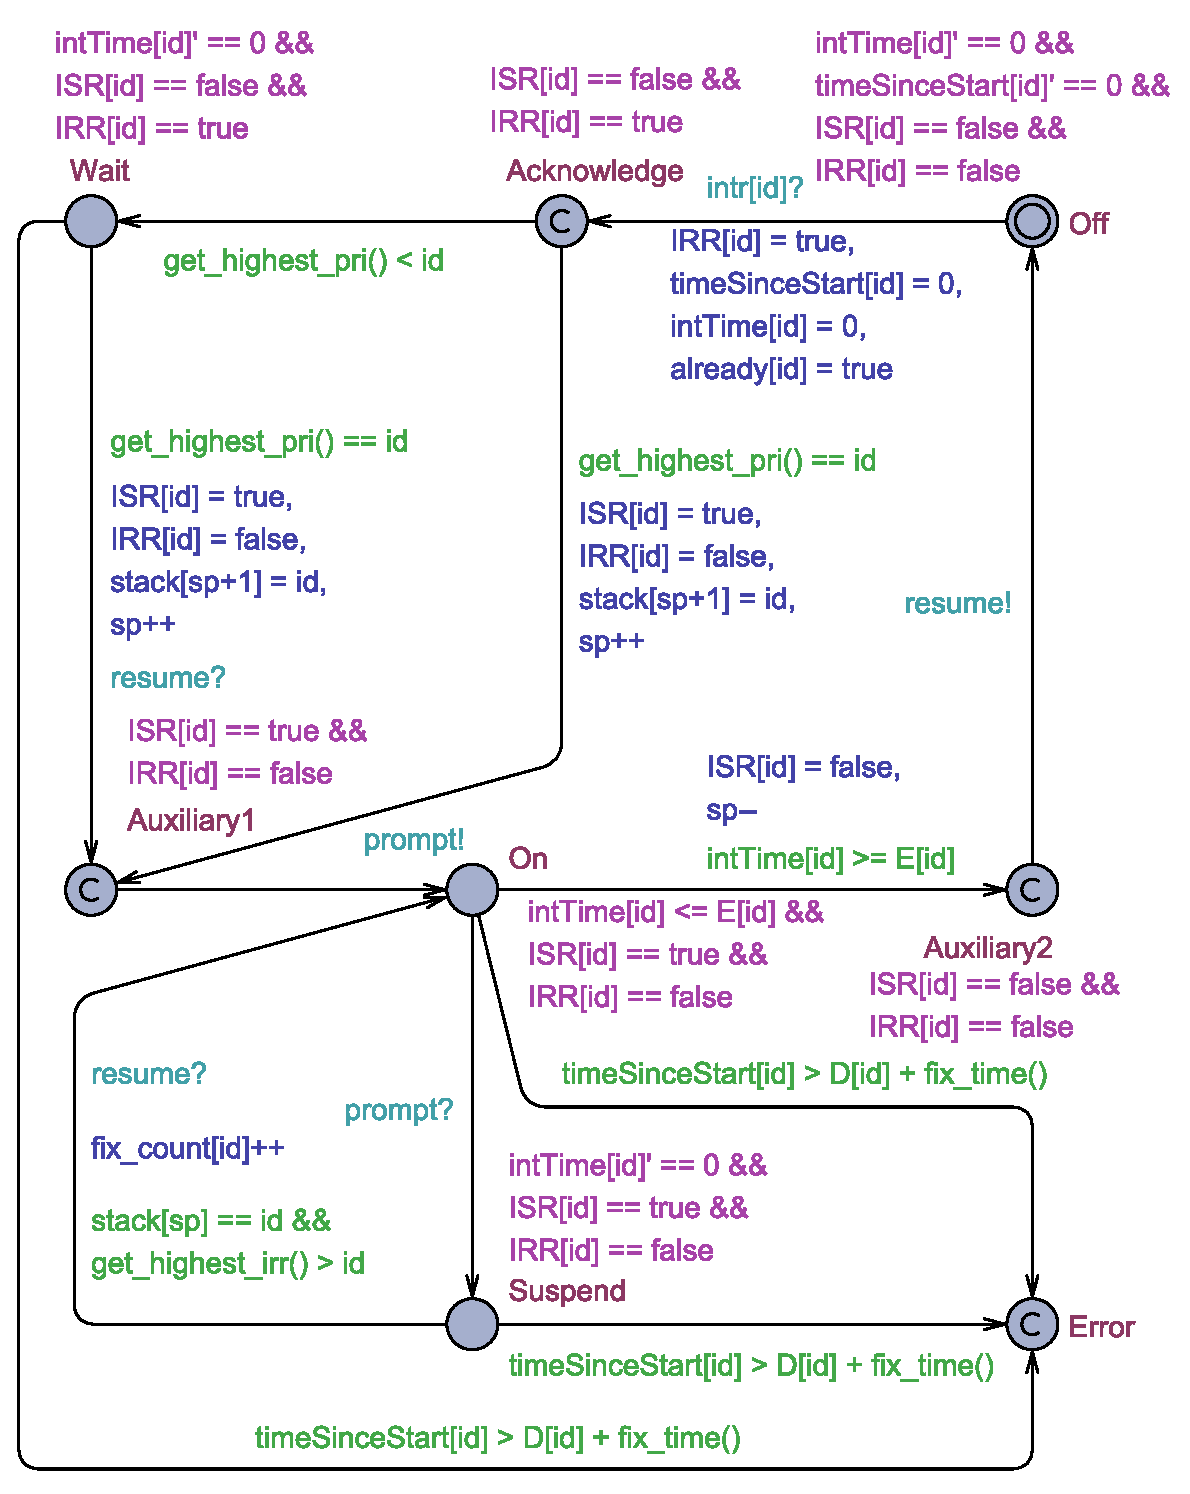
\includegraphics[width=0.9\textwidth]{Interrupt}
	\caption{某航空控制系统中断模型:普通中断}
	\label{fig:exp_intr}
\end{figure}

\begin{longtabu} to \linewidth {p{5em}p{5em}p{13em}X}
	\caption{某航空控制系统普通中断模板:位置}
	\label{tab:exp_intr_loc}\\
	\toprule[1.5pt]
	{\heiti 名称} & {\heiti 附加属性} & {\heiti 约束} & {\heiti 含义}\\
	\midrule[1pt]
	\endfirsthead
	\multicolumn{4}{c}{续表~\thetable\hskip1em 某航空控制系统普通中断模板:位置}\\
	\toprule[1.5pt]
	{\heiti 名称} & {\heiti 附加属性} & {\heiti 约束} & {\heiti 含义}\\
	\midrule[1pt]
	\endhead
	\hline
	\multicolumn{4}{r}{续下页}
	\endfoot
	\endlastfoot
	Off & 初始位置 & intTime和timeSinceStart保持静止,ISR和IRR对应位为false & 
	初始位置,当前没有该中断\\
	\midrule[0.5pt]
	Acknowledge & 关键位置 & ISR对应位为false,IRR对应位为true & 中断控制器
	接收到中断信号\\
	\midrule[0.5pt]
	Wait & & intTime保持静止,ISR对应位为false, IRR对应位为true & 当前有优先
	级更高的中断在运行,本中断等待。\\
	\midrule[0.5pt]
	Auxiliary1 & 关键位置 & ISR对应位为true,IRR对应位为false & 为表达Wait和
	Acknowledge到On的语义设置的辅助位置\\
	\midrule[0.5pt]
	On & & intTime不超过E[id](中断处理时间$T$),ISR对应位为true,IRR对
	应位为false & 中断正在被处理 \\
	\midrule[0.5pt]
	Suspend & & intTime静止,ISR对应位为true,IRR对应位为false & 中断被更高
	优先级的中断抢占CPU \\ 
	\midrule[0.5pt]
	Auxiliary2 & 关键位置 & ISR对应位为false,IRR对应位为false & 为表达On到
	Off的完整语义设置的辅助位置\\
	\midrule[0.5pt]
	Error & 关键位置 &  & 中断未在中断响应时间上限之内完成\\
	\bottomrule[1.5pt]
\end{longtabu}

\begin{longtabu} to \linewidth {p{5em}p{5em}XXXX}
	\caption{某航空控制系统普通中断模板:变迁 }
	\label{tab:exp_intr_mov}\\
	\toprule[1.5pt]
	{\heiti 迁出位置} & {\heiti 迁入位置} & {\heiti 条件} & {\heiti 同步} & 
	{\heiti 更新} & {\heiti 含义}\\
	\midrule[1pt]
	\endfirsthead
	\multicolumn{6}{c}{续表~\thetable\hskip1em 某航空控制系统普通中断模板:变迁}\\
	\toprule[1.5pt]
	{\heiti 迁出位置} & {\heiti 迁入位置} & {\heiti 条件} & {\heiti 同步} & 
	{\heiti 更新} & {\heiti 含义}\\
	\midrule[1pt]
	\endhead
	\hline
	\multicolumn{6}{r}{续下页}
	\endfoot
	\endlastfoot
	Off & Acknowledge & & 接收到中断信号 & IRR对应位置位,时钟清零 & 中断控
	制器接收到中断信号\\
	\midrule[0.5pt]
	Acknowledge & Wait & 本中断优先级不是最高 & & & 当前有更高优先级的中断存
	在,本中断等待\\
	\midrule[0.5pt]
	Wait & Auxiliary1 & 本中断优先级最高 & 接收到resume信号 & IRR对应位复位,
	ISR对应位置位,本中断入栈 &  高优先级的中断执行完毕,本中断得到CPU\\
	\midrule[0.5pt]
	Acknowledge & Auxiliary1 & 本中断优先级最高 & & IRR对应位复位,ISR对应位
	置位,本中断入栈 & 本中断优先级最高,准备执行\\
	\midrule[0.5pt]
	Auxiliary1 & On & & 发送prompt信号 & & 当前中断获得CPU,打断其他正在被处
	理的中断\\
	\midrule[0.5pt]
	On & Suspend & & 接收到prompt信号 & & 当前中断被更高优先级的中断打断\\
	\midrule[0.5pt]
	Suspend & On & 本中断在栈顶且无更高优先级的中断处在Wait位置 & 接收到resume
	信号 & fix\_count增加 & 高优先级的中断执行完毕,本中断得到CPU\\
	\midrule[0.5pt]
	On & Auxiliary2 & intTime[id]达到E[id] & & ISR对应位复位,本中断出栈 & 
	中断执行结束\\
	\midrule[0.5pt]
	Auxiliary2 & Off & & 发送resume信号 & & 通知其他中断获取CPU\\
	\midrule[0.5pt]
	Wait & Error & 中断响应时间超过上限 & & & 中断处理超时\\
	\midrule[0.5pt]
	On & Error & 中断响应时间超过上限 & & & 中断处理超时\\
	\midrule[0.5pt]
	Suspend & Error & 中断响应时间超过上限 & & & 中断处理超时\\
	\bottomrule[1.5pt]
\end{longtabu}

注意在Auxiliary2到Off的变迁中,时钟没有清零。这是因为在~\ref{subsubsec:exp_env} 
小节中的中断源需要用到intTime[id]时钟里的数据来表达中断触发的时序关系。

\subsubsection{AD中断模板}
\label{subsubsec:exp_ad}

AD中断是一个特殊的中断。它与~\ref{subsec:segment} 小节中提到的分段中断
类似,也是一个分段中断。然而它的分段的实现并非依赖一个类似于eCos那样完整的机制,
而是在中断自身调用特殊指令EOI清除了中断服务位,即将ISR寄存器对应位复位。这样做并
不会立即跳转其他中断去执行,之前被AD中断抢占的的其他中断依旧被抢占着。但是之后触
发的任何中断都会打断AD中断,抢占CPU。如果后来的中断优先级较低,那么就会造成优先
级反转。另外,在后来的中断运行结束之后,CPU会回到AD中断执行。尽管此时看ISR寄存器
的话,AD中断的对应位为0而有其他中断的对应位为1。因为恢复现场是按照退栈的顺序进行
的,这也是为什么我们在该模型中不得不引入一个栈。

除此以外,抽象时,我们将一个小周期内的连续多个AD中断看成了一个以减小状态空间,那
么一个AD中断内部的变迁就需要变得复杂一些。由于原本每个AD中断被分成了两部分,在模
型中的AD中断执行就会被分成$2\times c$段。

AD中断的状态机如图~\ref{fig:exp_AD} 所示。AD的参数只有中断ID,内部声明只有一个
用来计数的count。AD中断的位置和变迁说明分别见表~\ref{tab:exp_AD_loc} 和
表~\ref{tab:exp_AD_mov} 。

\begin{figure}[H]
	\centering
	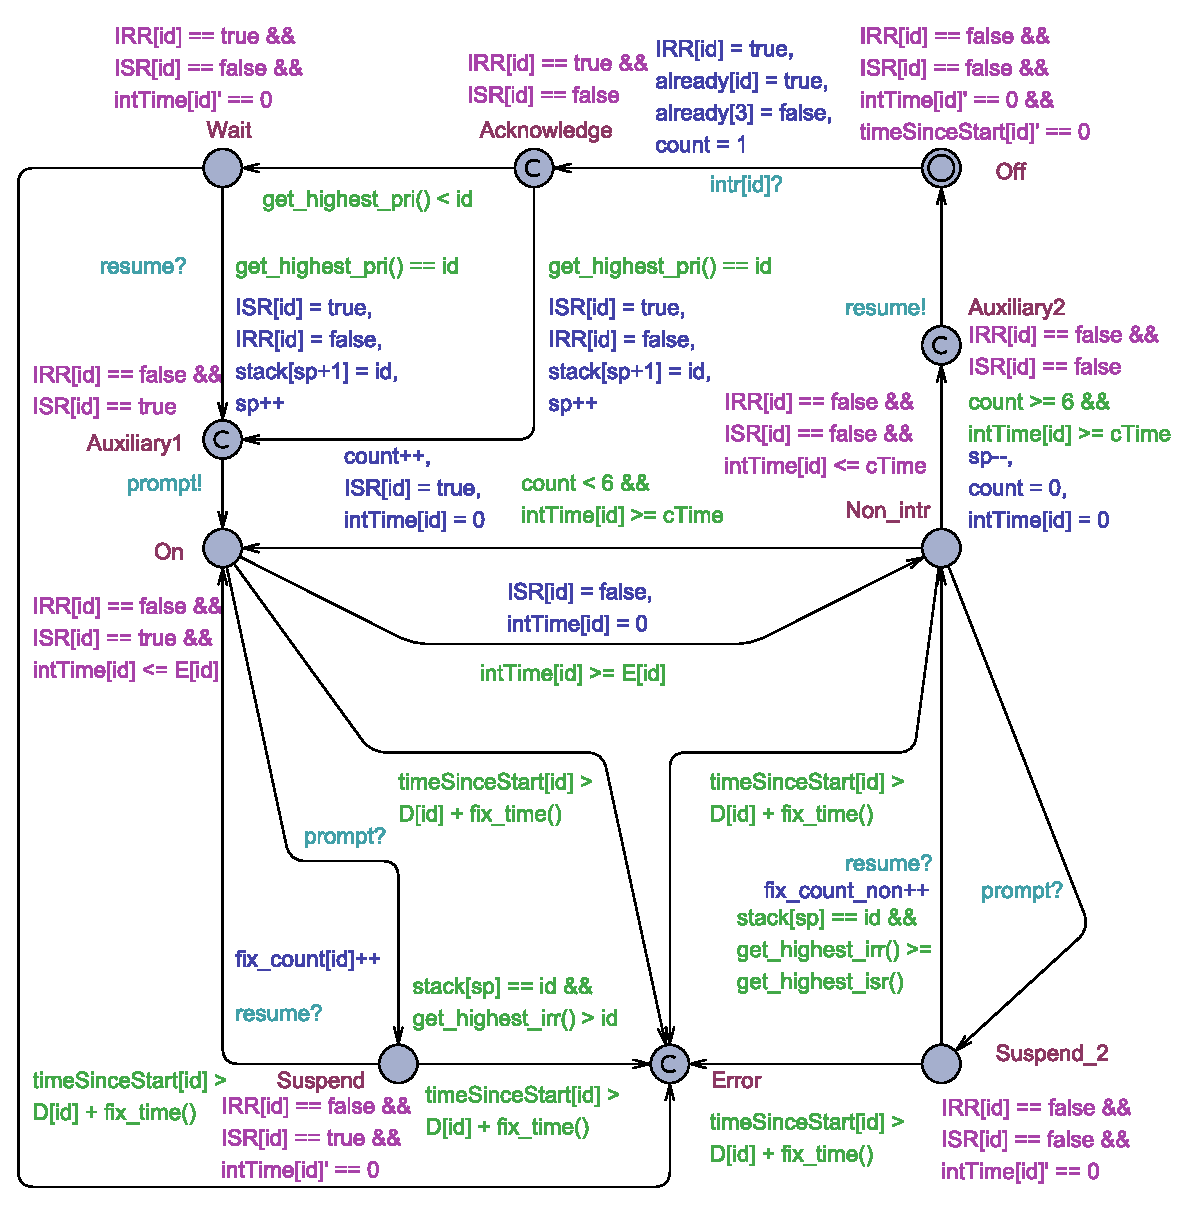
\includegraphics[width=\textwidth]{AD}
	\caption{某航空控制系统中断模型:AD中断}
	\label{fig:exp_AD}
\end{figure}

\begin{longtabu} to \linewidth {p{5em}p{5em}p{13em}X}
	\caption{某航空控制系统AD中断模板:位置}
	\label{tab:exp_AD_loc}\\
	\toprule[1.5pt]
	{\heiti 名称} & {\heiti 附加属性} & {\heiti 约束} & {\heiti 含义}\\
	\midrule[1pt]
	\endfirsthead
	\multicolumn{4}{c}{续表~\thetable\hskip1em 某航空控制系统AD中断模板:位置}\\
	\toprule[1.5pt]
	{\heiti 名称} & {\heiti 附加属性} & {\heiti 约束} & {\heiti 含义}\\
	\midrule[1pt]
	\endhead
	\hline
	\multicolumn{4}{r}{续下页}
	\endfoot
	\endlastfoot
	Off & 初始位置 & intTime和timeSinceStart保持静止,ISR和IRR对应位为false & 
	初始位置,当前没有该中断\\
	\midrule[0.5pt]
	Acknowledge & 关键位置 & ISR对应位为false,IRR对应位为true & 中断控制器
	接收到中断信号\\
	\midrule[0.5pt]
	Wait & & intTime保持静止,ISR对应位为false, IRR对应位为true & 当前有优先
	级更高的中断在运行,本中断等待。\\
	\midrule[0.5pt]
	Auxiliary1 & 关键位置 & ISR对应位为true,IRR对应位为false & 为表达Wait和
	Acknowledge到On的语义设置的辅助位置\\
	\midrule[0.5pt]
	On & & intTime不超过E[id](EOI之前的中断处理时间$T_{before}$),ISR对应位
	为true,IRR对应位为false & EOI之前,中断正在被处理\\
	\midrule[0.5pt]
	Suspend & & intTime静止,ISR对应位为true,IRR对应位为false & EOI之前,中
	断被更高优先级的中断抢占CPU \\ 
	\midrule[0.5pt]
	Non\_intr & & intTime不超过cTime(EOI之后的中断处理时间$T_{after}$),
	ISR对应位为false,IRR对应位为false & EOI之后,中断正在被处理\\
	\midrule[0.5pt]
	Suspend\_2 & & intTime静止,ISR对应位为false,IRR对应位为false & EOI之
	后,中断被其他中断抢占CPU \\
	\midrule[0.5pt]
	Auxiliary2 & 关键位置 & ISR对应位为false,IRR对应位为false & 为表达Non\_intr
	到Off的完整语义设置的辅助位置\\
	\midrule[0.5pt] 
	Error & 关键位置 &  & 中断未在中断响应时间上限之内完成\\
	\bottomrule[1.5pt]
\end{longtabu}

\begin{longtabu} to \linewidth {p{5em}p{5em}XXXX}
	\caption{某航空控制系统AD中断模板:变迁 }
	\label{tab:exp_AD_mov}\\
	\toprule[1.5pt]
	{\heiti 迁出位置} & {\heiti 迁入位置} & {\heiti 条件} & {\heiti 同步} & 
	{\heiti 更新} & {\heiti 含义}\\
	\midrule[1pt]
	\endfirsthead
	\multicolumn{6}{c}{续表~\thetable\hskip1em某航空控制系统AD中断模板:变迁}\\
	\toprule[1.5pt]
	{\heiti 迁出位置} & {\heiti 迁入位置} & {\heiti 条件} & {\heiti 同步} & 
	{\heiti 更新} & {\heiti 含义}\\
	\midrule[1pt]
	\endhead
	\hline
	\multicolumn{6}{r}{续下页}
	\endfoot
	\endlastfoot
	Off & Acknowledge & & 接收到中断信号 & IRR对应位置位,时钟清零,计数器启
	动 & 中断控制器接收到中断信号\\
	\midrule[0.5pt]
	Acknowledge & Wait & AD中断优先级不是最高 & & & 当前有更高优先级的中断存
	在,AD中断等待\\
	\midrule[0.5pt]
	Wait & Auxiliary1 & AD中断优先级最高 & 接收到resume信号 & IRR对应位复位,
	ISR对应位置位,AD中断入栈 &  高优先级的中断执行完毕,AD中断得到CPU\\
	\midrule[0.5pt]
	Acknowledge & Auxiliary1 & AD中断优先级最高 & & IRR对应位复位,ISR对应位
	置位,AD中断入栈 & AD中断优先级最高,准备执行\\
	\midrule[0.5pt]
	Auxiliary1 & On & & 发送prompt信号 & & AD中断获得CPU,打断其他正在被处理
	的中断\\
	\midrule[0.5pt]
	On & Suspend & & 接收到prompt信号 & & EOI之前,AD中断被更高优先级的中断打
	断\\
	\midrule[0.5pt]
	Suspend & On & AD中断在栈顶且无更高优先级的中断处在Wait位置 & 接收到resume
	信号 & fix\_count增加 & 高优先级的中断执行完毕,AD中断得到CPU\\
	\midrule[0.5pt]
	On & Non\_intr & intTime[id]达到E[id] & & ISR对应位复位,intTime[id]清
	零 & 中断执行到EOI\\
	\midrule[0.5pt]
	Non\_intr & On & intTime[id]达到cTime且计数器小于c & & 计数器加1,ISR对
	应位置位,intTime[id]时钟清零 & EOI之后,AD中断执行完且执行不足c次,执行
	下一次\\ 
	\midrule[0.5pt]
	Non\_intr & Suspend\_2 & & 接收到prompt信号 & & EOI之后,AD中断被其他中
	断打断\\
	\midrule[0.5pt]
	Suspend\_2 & Non\_intr & AD中断在栈顶且当前无其他中断可以抢占CPU & 接收
	到resume信号 & fix\_count增加 & 抢占AD的中断及之后的其他中断执行完毕,AD
	中断得到CPU\\
	\midrule[0.5pt]
	Non\_intr & Auxiliary & intTime[id]达到cTime且计数器达到c & & 计数器清
	零,intTime[id]时钟清零,AD中断出栈 & EOI之后,AD中断执行完且执行达到c次,
	退出中断\\ 
	\midrule[0.5pt]
	Auxiliary2 & Off & & 发送resume信号 & & 通知其他中断获取CPU\\
	\midrule[0.5pt]
	Wait & Error & 中断响应时间超过上限 & & & 中断处理超时\\
	\midrule[0.5pt]
	On & Error & 中断响应时间超过上限 & & & 中断处理超时\\
	\midrule[0.5pt]
	Suspend & Error & 中断响应时间超过上限 & & & 中断处理超时\\
	\midrule[0.5pt]
	Non\_intr & Error & 中断响应时间超过上限 & & & 中断处理超时\\
	\midrule[0.5pt]
	Suspend\_2 & Error & 中断响应时间超过上限 & & & 中断处理超时\\
	\bottomrule[1.5pt]
\end{longtabu}

\subsubsection{环境模板}
\label{subsubsec:exp_env}

环境模板本身并不复杂,但是需要表达出中断的时序关系。在本项目中,中断并不是随机
触发的。除了前文提到的定时中断和通讯中断以外,还有一条时序约束,即在每个小周期
内,3号中断执行了固定之后才会触发AD中断。环境模板的状态机用不同的变迁表示了这
些中断的触发时序关系,如图~\ref{fig:exp_env} 所示。

在这个模板中,位置只有一个且没有实际意义。图中的变迁中都表达了,随机选择一个中
断号,触发该中断并将中断计数器减少1。在所有变迁条件中都要求对应中断计数器大于0。
对于0号和1号中断,它们是通讯中断,因此条件是它们从未触发过或者距离上一个触发超
过了$T^\prime$。对于3号中断,它是一个小周期中断。在整个大周期中,会有多个小周
期,因此每个周期才能触发一个3号中断。对于2号中断,它只能在3号中断执行了固定之
后触发。对于剩下的456号中断,因为只会触发一次且无其他约束,因此可在任意时刻触
发。

\begin{figure}[H]
	\centering
	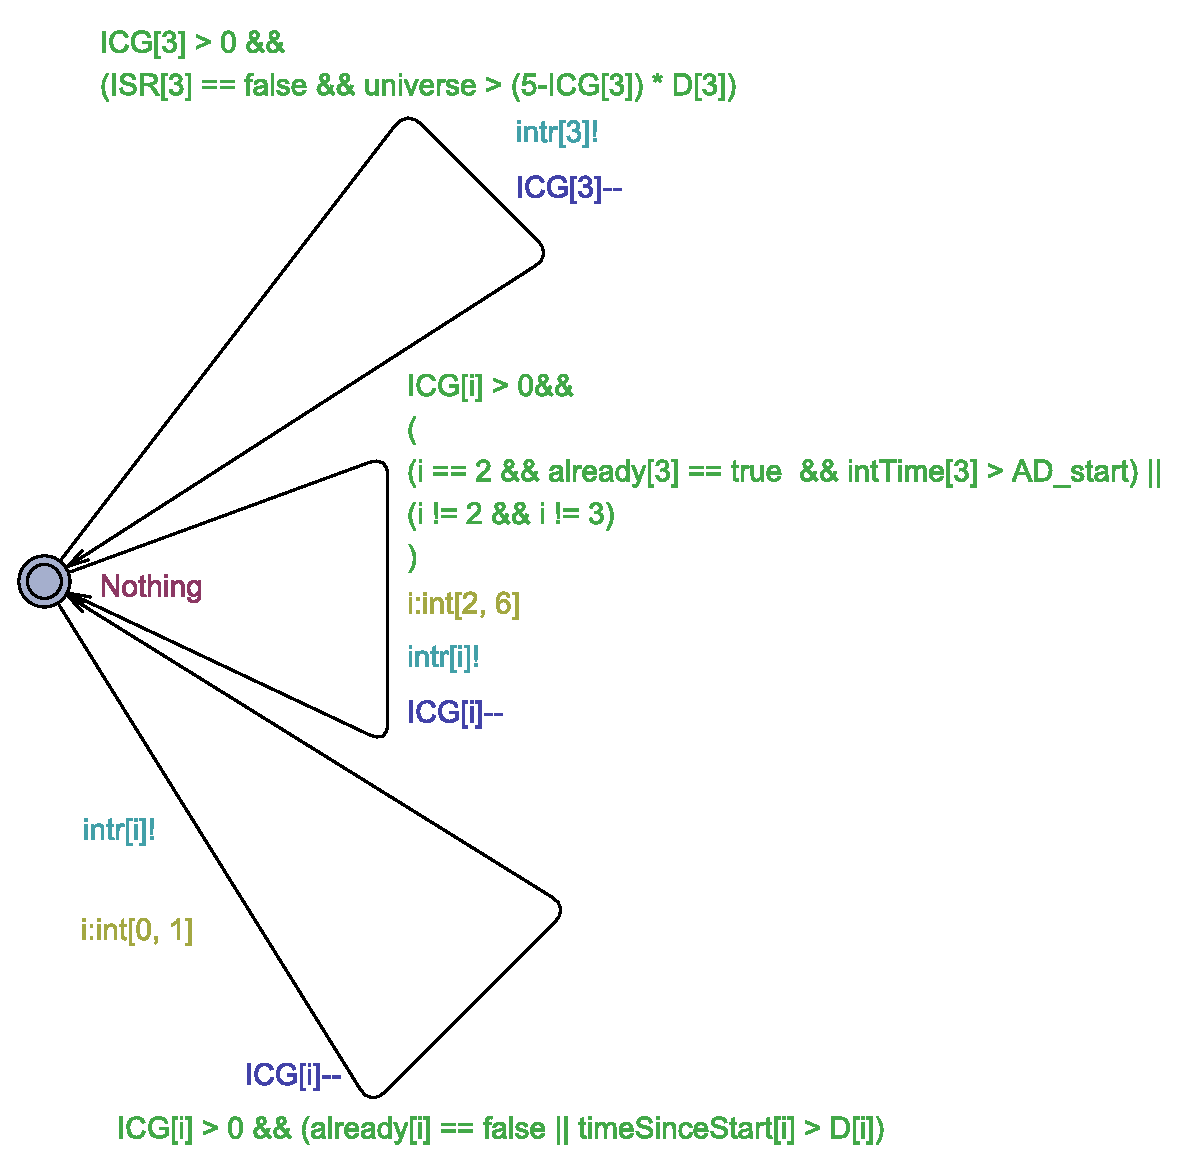
\includegraphics[width=0.8\textwidth]{env}
	\caption{某航空控制系统中断模型:环境模板}
	\label{fig:exp_env}
\end{figure}

\subsubsection{系统声明}
\label{subsubsec:exp_model_decl}

系统声明很简单,如图~\ref{fig:exp_model_decl} 所示。在此不赘述。

\begin{figure}[H]
	\centering
	\begin{lstlisting}
	intr0 = Interrupt(0);
	intr1 = Interrupt(1);
	intr2 = AD(2);
	intr3 = Interrupt(3);
	intr4 = Interrupt(4);
	intr5 = Interrupt(5);
	intr6 = Interrupt(6);
	environment = env();
	system intr0, intr1, intr2, intr3, 
		intr4, intr5, intr6, environment
	\end{lstlisting}
	\caption{某航空控制系统中断模型:系统声明}
	\label{fig:exp_model_decl}
\end{figure}

\section{分析与验证}
\label{sec:experiment}

在构建完模型之后,我们用\uppaal 提供的模拟器和验证对模型进行分析验证。首先,我们
对性质~\ref{property:all} 尝试验证。性质~\ref{property:all} 表示所有中断都不
会进入Error位置,即所有中断均不会超时。

\begin{property}
	A[] not (intr0.Error || intr1.Error || intr2.Error || intr3.Error 
	|| intr4.Error || intr5.Error || intr6.Error) 
	\label{property:all}
\end{property}

然而,该性质验证失败,反例如图~\ref{fig:exp_counter} 所示。我们跟随该反例复原
一下执行流程。首先3号中断触发,没有其他任何干扰因素,3号中断运行至结束。此时2号
中断,即AD中断触发条件满足,AD中断触发。AD中断执行到EOI指令之后,ISR对应位复位,
此时IRR和ISR所有为均为0,栈内只有AD中断。此时,4号中断触发,抢占CPU。此时,栈内
4号中断在AD中断之上,也就是说在4号中断执行结束之前,AD中断会被一直阻塞。由于
$T_4>T^\prime_2$,因此,AD中断会超时。在与合作方工程师交流之后,我们一致认为在
系统这种中断触发序列是有可能的。避免方式也很简单,只要将4号中断的触发时机提前,
保证其在AD执行到EOI之前触发即可。

\begin{property}
	A[] not (intr0.Error || intr1.Error || intr3.Error || intr4.Error || 
	intr5.Error || intr6.Error) 
	\label{property:some}
\end{property}

接着我们尝试验证AD中断之外的其他中断的实时性。经过尝试,性质~\ref{property:some}
在消耗数小时后报告内存溢出,验证中止。这个结果在意料之中,因为在~\ref{subsubsec:exp_decl} 
小节的定义中,我们可以看到0号中断总共可以触发50次,这会极度增大状态空间,内存
溢出是正常。在尝试了各种办法之后,只有在将0号中断的数量修改到5以下,\uppaal 才会
给出验证结果\pozhehao 验证通过。

\begin{figure}[H]
	\centering
	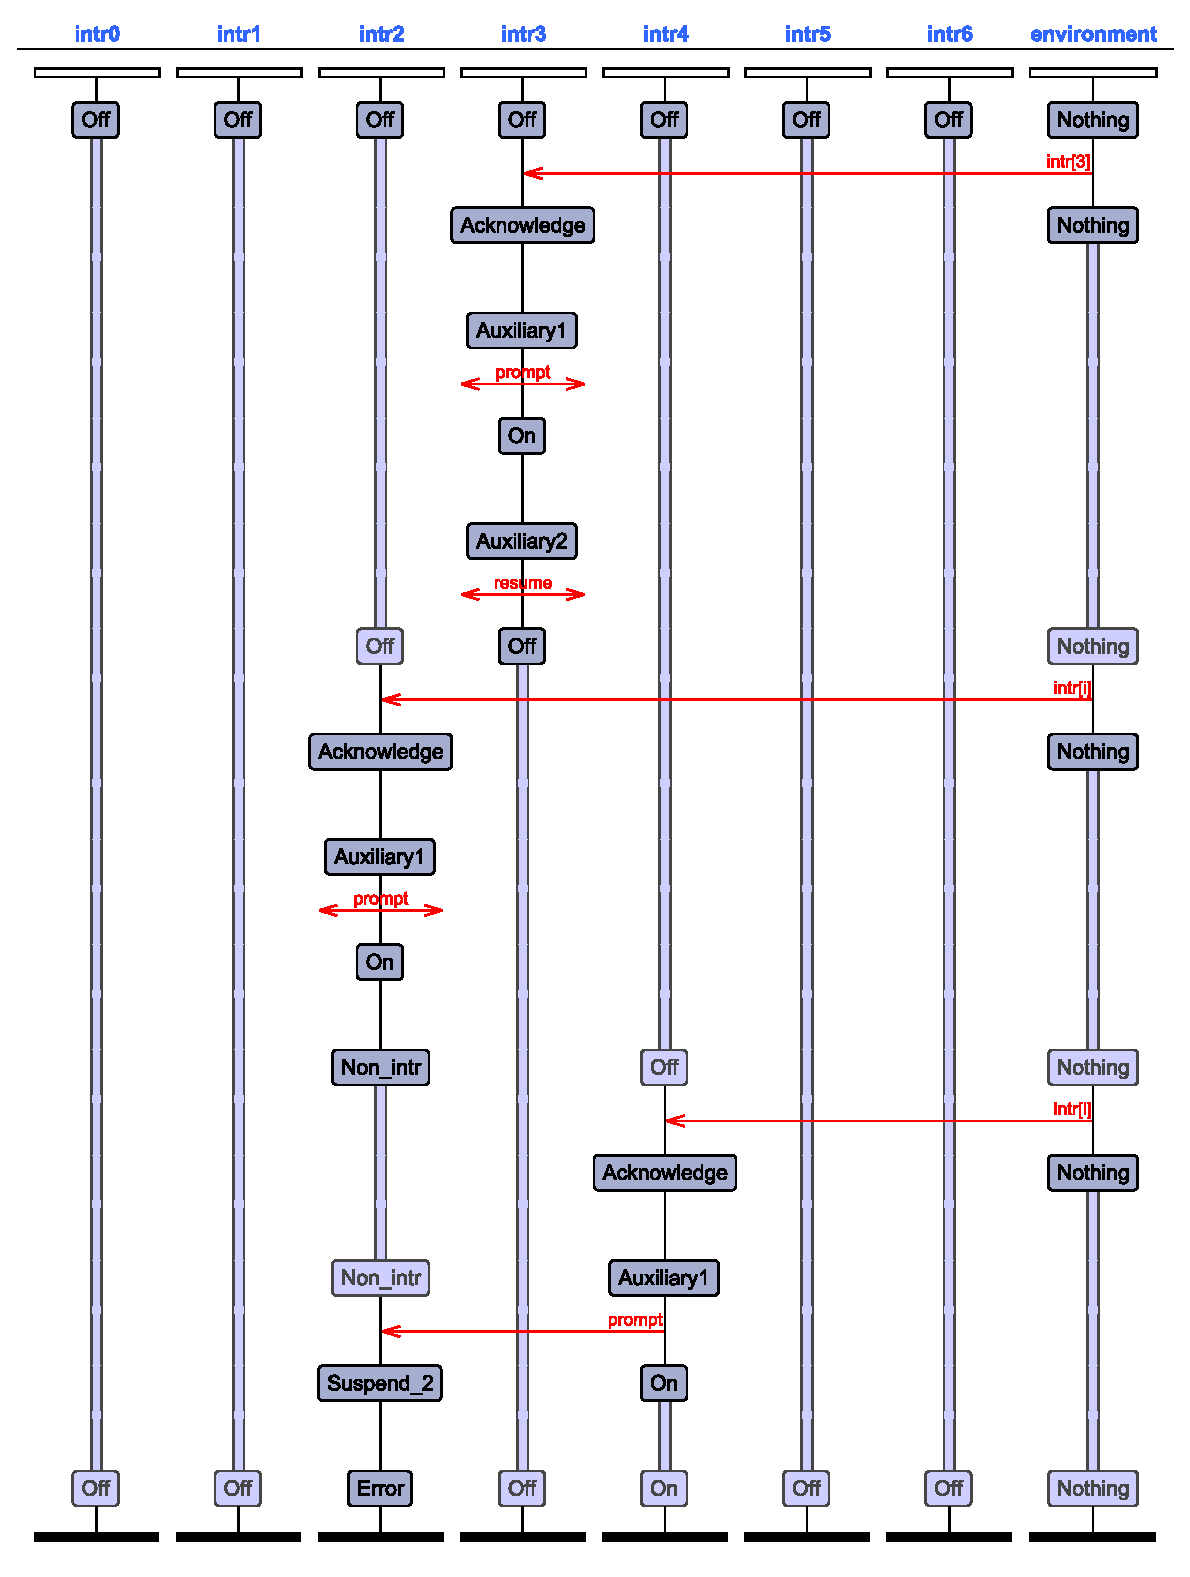
\includegraphics[width=\textwidth]{msc}
	\caption{性质~\ref{property:all} 的反例}
	\label{fig:exp_counter}
\end{figure}

\section{本章小结}
\label{sec:sum_4}

本章结合实际项目,对某航空控制系统上的中断驱动程序进行分析,对其中断设置在\uppaal 
中构建了形式化模型,然后对其实时性属性进行分析和验证。该工作成功找出一个可能违反
中断实时性要求的反例,并与对方工程师交流得到确认。

本章描述的应用过程符合第~\ref{cha:intr} 章中提出的方法。在该航空控制系统上
的中断驱动程序中,普通中断基本上直接套用了第~\ref{cha:intr} 章中的基本中断模型,
而AD中断由于其极端的特殊性,并不能直接套用前述模型。因此,在构建AD中断模型时,本
章完全按照上文提到的方法,并在最后构建自动机时借鉴了分段中断的构建思想。

由此可见,本文第~\ref{cha:intr} 章中提出的面向嵌入式程序里中断实时性研究的方法
以及总结出的相关形式化模型在这个问题中具有良好的指导和借鉴意义。